Das auf Angular basierende Frontend spiegelt die unterschiedlichen Ansätze wieder und stellt zusätzlich Tools zur Verfügung.

\subsection{NER-Ansatz}

Der \gls{ner}-Ansatz basiert auf einem selbst antrainierten und programmierten Modell und ermöglicht sowohl das Aufbereiten der Daten als auch das Extrahieren der Daten aus einer Rechnung. Daher werden diese zwei Schritte unterteilt in: 

\begin{itemize}
    \item NER Annotation Tool
    \item Invoice Reader
\end{itemize}

\subsubsection{NER Annotation Tool}

Bei dem NER Annotation Tool handelt es sich um ein selbst programmiertes Tool, welches es einem erleichtert, Rechnungen oder übliche Texte im pdf-Format zu klassifizieren. 

\begin{figure}[H]
    \centering
    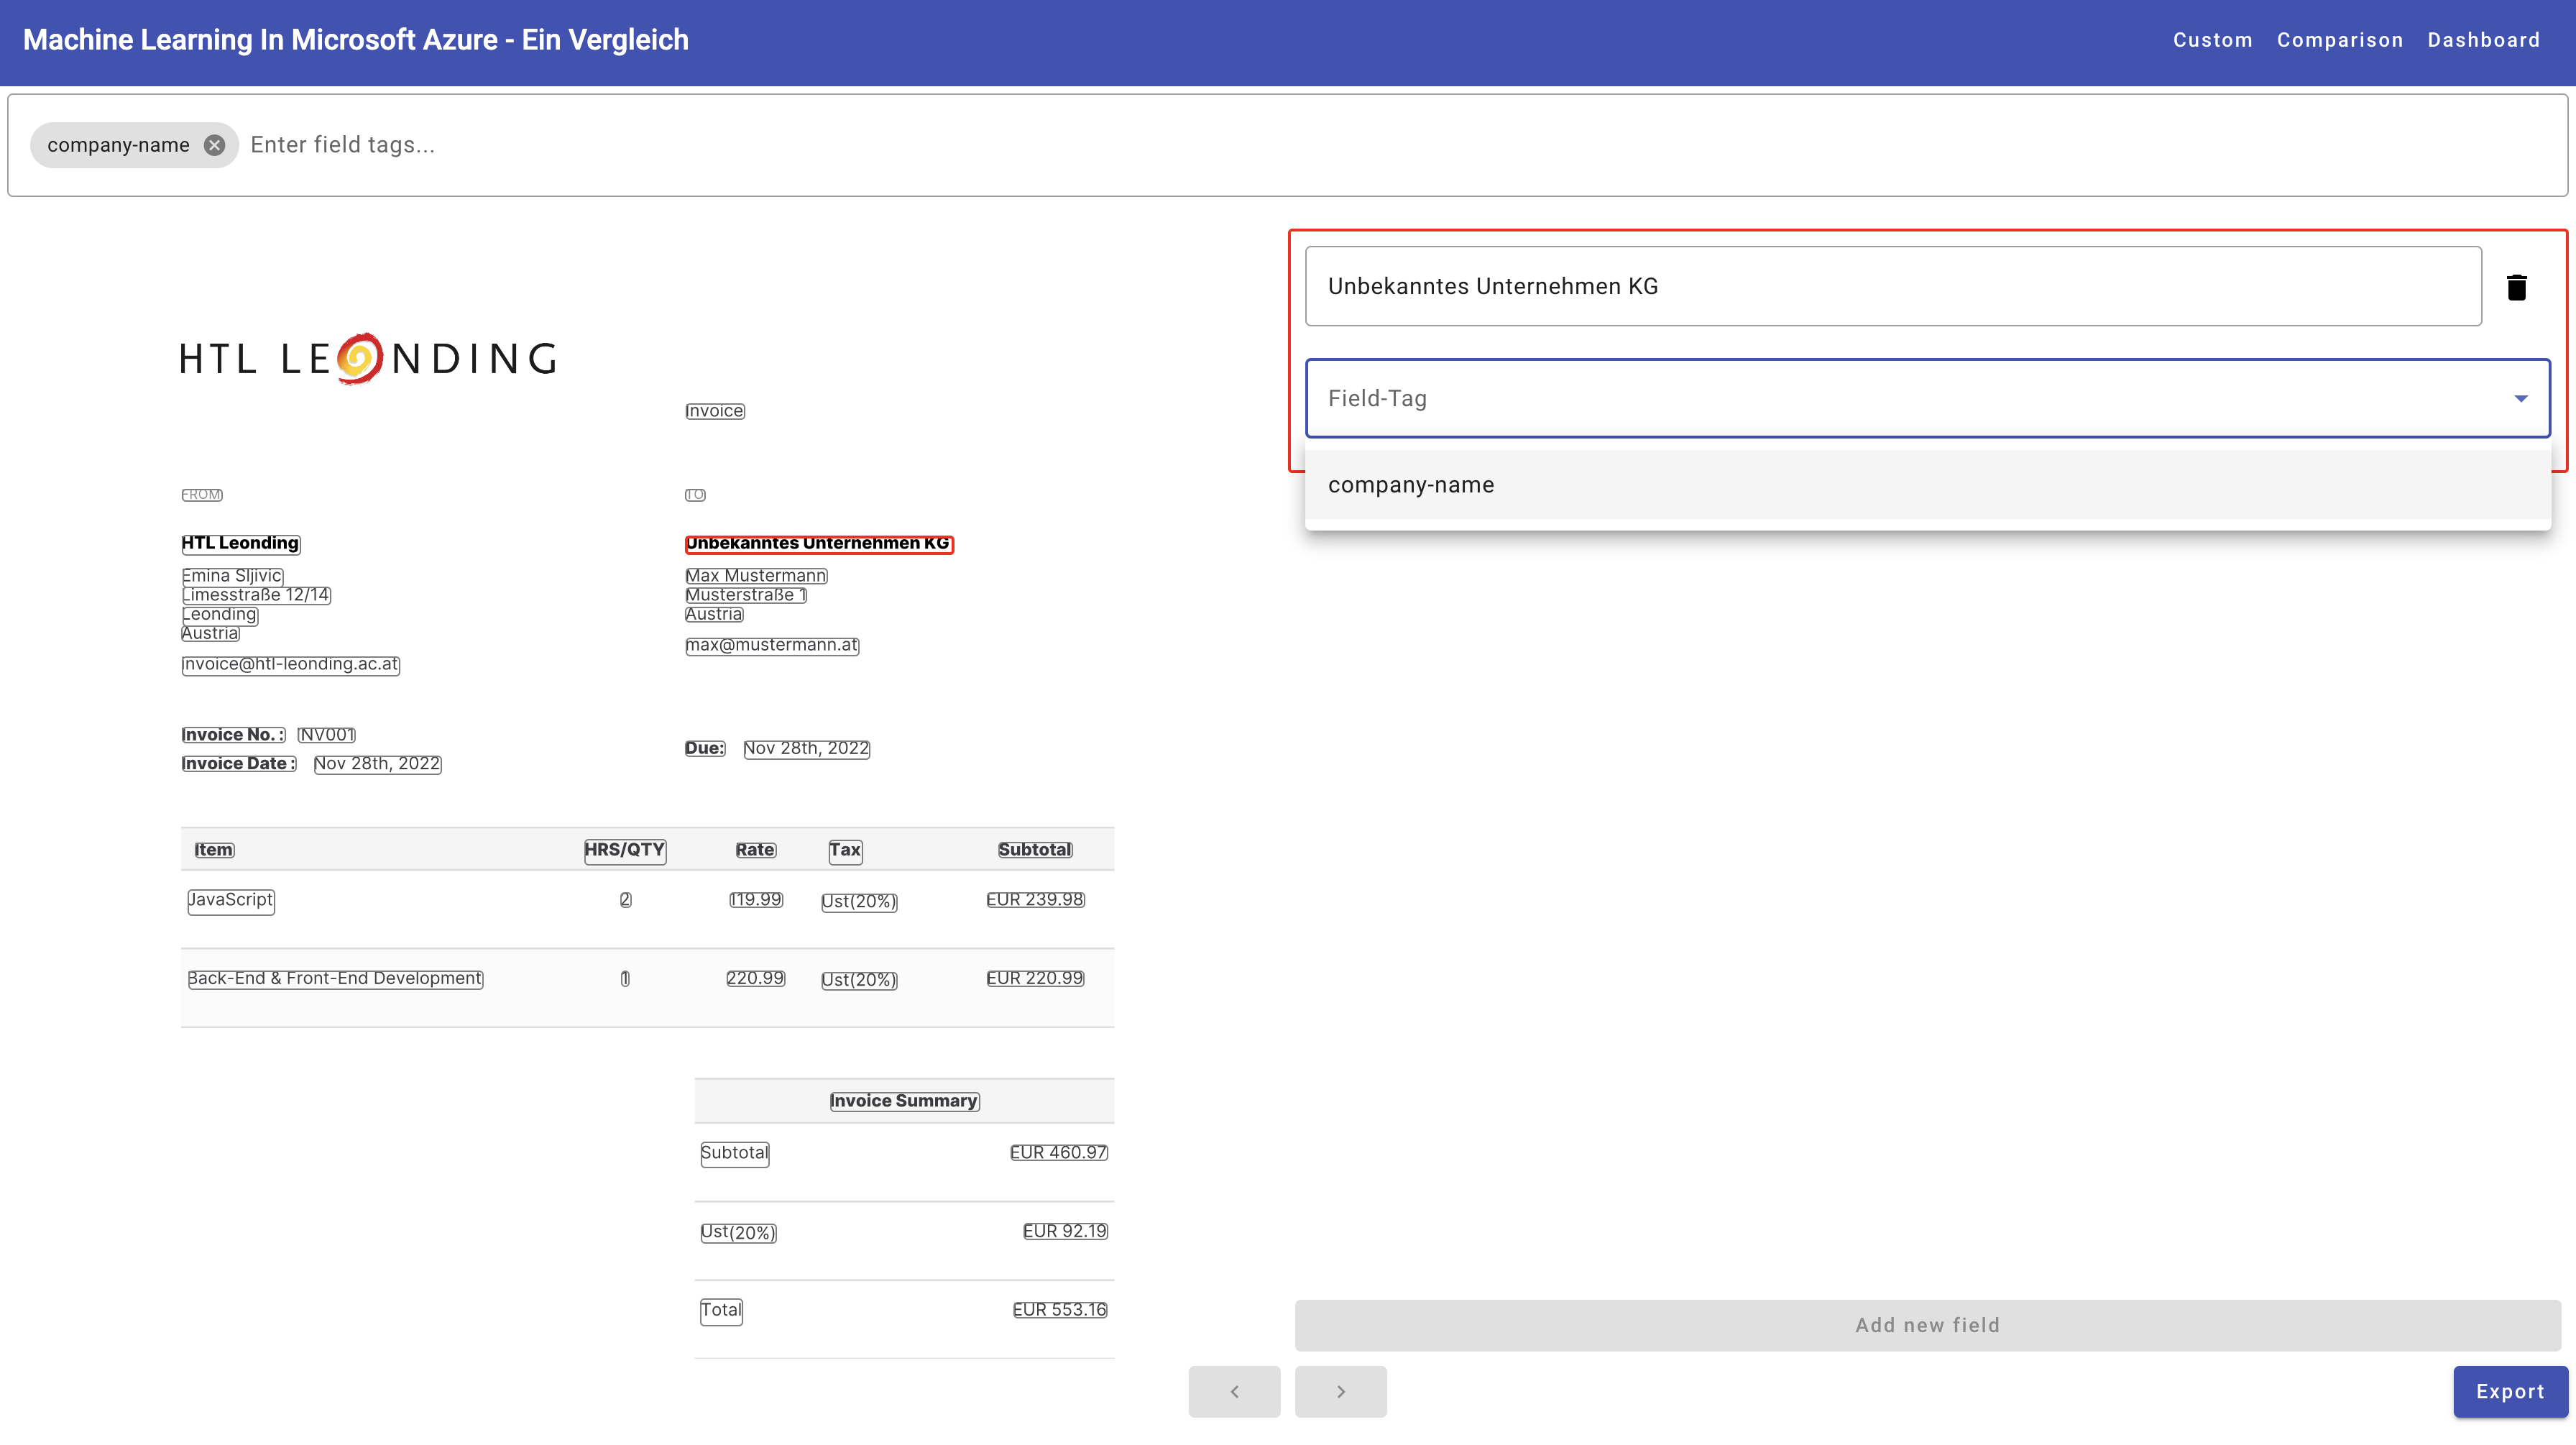
\includegraphics[scale=0.25]{sections/implementation/images/NERAnotationTool.png}
    \caption{NER Annotation Tool mit Beispieldaten}
\end{figure}

Nachdem der User eine oder mehrere Dateien ausgewählt hat, wird im Hintergrund mithilfe von Event-Binding eine Methode ausgelöst, die entweder einen oder mehrere \gls{http}-GET-Requests abschickt. Diese werden als Promise gespeichert, was heißt, dass das Programm auf alle Antworten wartet, bevor es mit dem nächsten Schritt weiter macht. Die Antworten geben die ausgewählten pdf-Dateien als blob-Objekt zurück.

\begin{lstlisting}[language=TypeScript, caption = {HTTP-GET-Requests für die pdf-Dateien}]
    const getImagePromises = this.invoices.map(i => this.http.get(i.url, {responseType: 'blob'}).toPromise());
    const images = await Promise.all(getImagePromises);
\end{lstlisting}

Dieses blob-Objekt wird durch das zusätzlich installierte Paket \lstinline{ng2-pdf-viewer} dargestellt. 

Mit weiteren \gls{http}-Requests werden die Azure Functions aufgerufen, um das pdf-File richtig zu skalieren und um jede Wortgruppe mit einer Box zu umranden. Mithilfe dieser Boxen kann die Rechnung annotiert werden. Jede Annotation besteht aus dem Inhalt der Box und einer Entität, die zuvor im oberen Feld eingegeben wurden. 

Um diese Boxen darzustellen, wird automatisch ein \lstinline{div}-Element über dem pdf-Viewer erstellt und durch den \lstinline{renderer} mit den Boxen gefüllt. Ein \lstinline{renderer} ermöglicht das Eingreifen in den \gls{html}-Struktur über den dahinterliegenden Code.

All diese \gls{http}-Requests werden mit dem über Dependency-Injection initialisierten HttpClient ausgeführt. Dieser Client wird von Angular zur Verfügung gestellt.

Nachdem alle Rechnungen annotiert wurden, können die Annotationen im \lstinline{json}-Format über den 'Export'-Button exportiert werden.

\begin{lstlisting}[caption={Beispiel für eine exportierte json-Datei}]
    {
        "company-name": "Unbekanntes Unternehmen KG",
        "company-address": "Musterstrasse 1",
        "invoice-id": "INVOO01",
        "invoice-date": "Nov 28th, 2022",
        "item-header": "Item",
        "qty-header": "HRS/QTY",
        "rate-header": "Rate",
        "total-header": "Subtotal",
        "total-value": "EUR 553.16"
    }
\end{lstlisting}

\subsubsection{Invoice Reader}

Der Invoice Reader ermöglicht das Extrahieren von Daten aus einer pdf-Datei, daraufhin werden diese Daten im Interface dargestellt.

\begin{figure}[H]
    \centering
    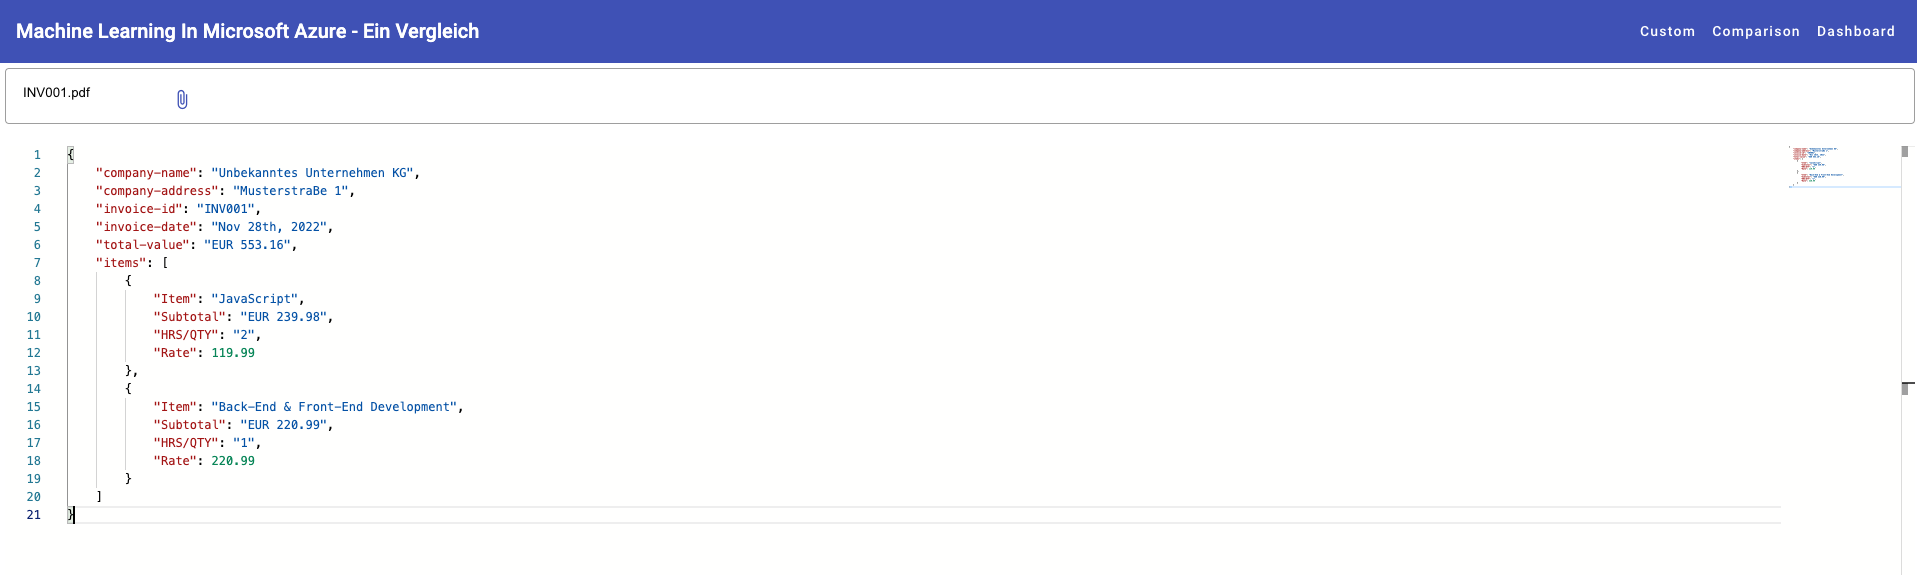
\includegraphics[scale=0.25]{sections/implementation/images/InvoiceReader.png}
    \caption{Invoice Reader mit Beispieldaten}
\end{figure}

Nachdem der User eine pdf-Datei auswählt, wird ein \gls{http}-Request an das Backend abgeschickt und als Antwort wird ein json-Objekt zurückgeliefert, welches die extrahierten Daten enthaltet. Diese Daten werden daraufhin formatiert und in einem monaco-Editor dargestellt.

